% !Mode:: "TeX:UTF-8"
% 调制技术与其它基带技术的研究

\chapter{分布式组网光通信系统的灯组调度}\label{chap:baseband-technology}
\section{引言}
对于一个安装有多个灯组的房间来说,为了保证用户和灯组之间的高效无缝的通信,需要设计一种灯组调度算法,来实现多用户的通信,并适应移动用户的移动性需求。
通常对于灯组的种类划分,可以分为两种,一种是实现均匀照明覆盖的灯组,这种灯组通过使用多个宽角度的LED芯片,使得每个LED灯组的覆盖范围较大。而另外一种是射灯照明的灯组,
这种灯组的方向性较为明显,其灯组的覆盖方位也较小[49]。在本章中,我们先研究第一种灯组室内组网的情况。本章将首先介绍分布式组网光通信系统的基本结构,
在给出本章提出的一种灯组调度算法,来解决该架构下移动用户的灯组调度问题。

\section{分布式组网光通信系统分析}
对于多个大覆盖范围的LED灯组的组成的室内光通信系统,为了保障对移动用户的支持,又避免实现复杂的灯组切换机制,本章采用了分布式的灯组组网布局。
这里的分布式是指所有的灯组的数据传输到受到调度器的控制,当调度器允许当前灯组和某用户进行通信时,所有的灯组将会发送相同的信息与该用户进行通信。
以一个房间内含有四个灯组为例,其分布式灯组网络架构如下图所示。

\begin{figure}[htbp]
    \centering
	\includegraphics[width=0.8\textwidth]{figures/chapter-4/DistributionOverView.eps}
	\caption{布式灯组网络架构}
	\label{fig:distribution-overview}
\end{figure}

图中,四个灯组和调度器相连,下图的圆圈表示的是灯组的覆盖面积,图中用户1处于灯组3的覆盖区域,用户2处于灯组3和灯组4的共同覆盖区域中。

\subsection{本文采用的上下行信道}
由于光通信系统上下行数据传输的不对称性,同时为了避免上行链路电路的复杂度,在本系统中下行使用光通信信道,上行使用红外信道进行数据传输。
红外通信作为一种最常见的室内短距离无线通信技术,早就在短距离通信中得到广泛地应用,其技术也已经较为成熟。本系统将光通信和红外通信相结合,既可以简化系统的复杂度,又可以保障系统的性能。其通信结构如下图所示。

\begin{figure}[htbp]
    \centering
	\includegraphics[width=0.8\textwidth]{figures/chapter-4/DistributionChannel.eps}
	\caption{分布式组网光通信系统采用的上下行信道}
	\label{fig:distribution-channel}
\end{figure}

在灯组侧,拥有光发射器和红外接收器,而在用户侧拥有光接收器和红外发射器,当灯组有数据需要发送给用户时,就使用光发射器将数据经过光信道发送出去,
而用户发送数据时,则使用红外发射器将数据发送出去。这样,由于上下行采用的是不同的信道,因此上下行通信互不影响,类似于采用频分复用进行上下行通信的系统。
在本系统中,由于所有的灯组都安装了红外接收器,并且一直处于打开的状态,因此,当用户通过红外发射器发送数据后,其周围的灯组都是可以接收并获得该用户的数据。

\subsection{多用户通信方式}
对于多个移动用户的场景,本系统采用的方式为基础的时分复用技术,即将用户安排在不同的时隙上进行用户的服务。
这种方式对室内的移动用户的数目有一定的要求,但是在常见的室内光通信系统中,尤其是常见的办公室和会议室,使用的用户数目一般都不会很多,因此,采用时分复用进行多用户通信是简单而又合理的。

由于在分布式组网条件下,灯组的作用相当于一根发送天线,用户的移动将不再受到灯组位置的制约,但是用户的移动将会影响到发送灯组集合的选择,所以,下面将讨论对于移动用户的灯组调度策略。

\subsection{分布式组网调度策略分析}
在实际的通信过程中,如果对于每一个用户而言,每次的通信可以直接使用房间内所有的灯组共同和用户进行数据传输,无疑是最为简单的方式,也不需要考虑用户在灯组的切换,但是这种方式会导致某些灯组发送的信息根本就不会被用户接收到,
从而造成大量的资源浪费。因此,需要一种合适的灯组调度算法,在分布式灯组组网的架构下,根据用户的移动中的需求分配相匹配的灯组资源。

传统的调度方法是使用下行信道广播灯组的信息,当用户接收到多个灯组的信息后,再通过上行传输,反馈接收到的灯组信息和信号强度信息给调度器,调度器通过此信息选择合适的灯组集,这种调度方式使得灯组的配置过程需要在上下行两个过程之后才能完成,影响数据的正常传输,耗费系统开销,
同时灯组集选择是依据当前的灯组接收信号强度来进行的,没有考虑到用户的移动情况。其中有一种调度方法是以灯组接收信号强度最大化为准则进行灯组的选取,这种方式能快速选择可使用灯组,却不能使用户得到多个灯组的协作,另一种方式是以灯组接收信号强度判决可服务的灯组作为灯组集服务用户,
这种方式引入了灯组间的协作,但是判决的依据只是当前的接收信号强度,从而得到的灯组调度结果有一定的局限性。在分布式灯组组网的条件下,可以通过合理地选择更加准确的灯组集合联合发送用户数据信息来解决这个问题,通过相邻灯组的协同工作,来保障用户在移动中的通信质量。

\section{基于运动方向的灯组协同调度}
\subsection{判决变量依据}
不同于上述提及的其他系统中使用上下行传递和反馈信息的方式来进行灯组的选择,本系统中测量的是数据传输中用户给灯组发送应答数据时的灯组接收功率。根据上述的信道介绍,上行采用的是红外信道,于是当用户采用红外信道上行发送灯组传输数据的应答信息时,
上方的多个灯组都有可能接收到用户的应答信息,此时灯组接收到的信号强度则可作为系统的灯组调度的输入参数。

使用上述方式,可以直接利用数据传输中的信息进行灯组的调度,从而可以避免造成额外的系统开销和操作复杂度。但是由于上下行的信道不对称性,收到用户应答信息的灯组并非就是可以给用户发送数据的灯组,所以当灯组接收到用户应答信息后,
仍然需要判别用户是否处于该灯组的覆盖范围内。判决的门限值为设定当用户处于光通信覆盖区边缘时在反向信道灯组接收到的接收信号强度,设该值为$P_{th}$。同时由于灯组接收到用户的信号强度是动态变化的,所以不能直接根据接收信号值大于$P_{th}$就认为可以使用该灯组为用户提供服务,
而应该使用迟滞判决方案,假设灯组$A_{i}$接收到用户数据的接收信号强度为$P_{i}$,则当其满足以下公式时,可以认为用户处于灯组$A_{i}$的覆盖范围内。

\begin{equation}
    P_{i}-P_{th} > P_{hy}
    \label{equ:user-enter-hy}
\end{equation}

其中,$P_{hy}$即为判决的迟滞门限值。

\subsection{用户的运动方向判别}
如果系统只知道灯组的接收信号强度信息,根据式()可以判决出当前可以为该用户服务的灯组集,从而使用这个灯组集为用户提供数据传输服务。
这种方式其实也就等效于上述提及的通过下行广播,再将接收到的广播的数据上行告诉调度器进行灯组调度的方式。但是这种方式会产生一定的问题,
如当用户的移动速率过快时,或者是调度的周期过长时,用户容易走到调度灯组集合的边缘区,甚至是离开当前灯组集的覆盖范围。比如说,当一个用户处于一个灯组的核心区时,
此时进行了灯组的调度,将为该用户的灯组确定只使用当前灯组,但是考虑到随着用户的移动,在下一个调度时刻来临时,有可能该用户已经移动到了该灯组的边缘或者移动出该灯组的覆盖范围了,
导致在该段调度时间内,该用户并没有被很好地服务到。

该现象发生的主要原因就是当系统进行灯组调度时,依据的是当前的灯组接收信号强度信息,因此得到的调度结果仅仅对当前时刻是最优的,并不能保证在整个调度时间的最优。
要想得到调度周期内的最优灯组调度,还需要知道用户的运动的趋势,这才可以使我们了解到将来可以覆盖到该用户的灯组,从而可以更好地为用户提供服务。
而对于该用户的运动方向信息的获取,我们可以从多次的灯组的接收信号强度中分析得到,因为灯组接收信号强度的变化可以反应一定的用户移动方向信息。

由于系统的反向链路使用的是红外信道,依据其传输模型[50],红外通信在自由空间中的$LOS$的路径损耗主要和用户和灯组之间的距离$d$和光传播到用户接收平面的入射角度和用户的接收视场角有关。
而当用户向上发送红外数据时,在用户附近的灯组在接收光功率的路径损耗,可以近似正比于用户和灯组之间距离的平方[51],接收电功率的路径损耗则可以近似正比于用户和灯组之间的距离的四次方,
因此类似于距离-路径损耗模型,可以通过下式根据参考值计算出某一灯组测量到的功率所对应该灯组和用户之间的距离值

\begin{equation}
    \frac{{{P_0}}}{{{P_i}}} = \frac{{\frac{1}{{d_0^4}}}}{{\frac{1}{{d_i^4}}}}
\end{equation}

其中$P_{0}$和$d_{0}$分别为灯组和用户之间的参考距离和参考功率,$P$和$d$为灯组测量到的电接收功率和所需要计算的灯组和用户之间的距离。假设灯组距离接收平面的高度$h$是已知的,那么此时可以获得用户距离某灯组$A_{i}$之间的水平距离

\begin{equation}
    {x_i} = \sqrt {d_i^2 - {h^2}}
\end{equation}

这样,利用某一个灯组在本次调度和上一次调度时刻分别接收到的信号强度$P_{ni}$和$P_{bi}$,就可以对应地求出本次调度和上一次调度时刻用户距离该灯组的水平距离$x_{ni}$和$x_{bi}$,进行可以使用该水平距离的差值 来描述该用户对于灯组$A_{i}$的运动趋势

\begin{equation}
    \Delta {x_i} = {x_{ni}} - {x_{bi}}
\end{equation}

当该值为正时,说明该用户正在远离灯组$A_{i}$,否则说明该用户正在靠近灯组$A_{i}$。
通过上述的分析,系统就可以在调度时刻,不仅能获得当前的用户反向接收信号强度信息,并且可以获得用户相当于各灯组的运动方向信息。

但是如果所有灯组信号强度$P_{ni}$和$P_{bi}$都相差较小时,这就说明当前用户在所在位置中运动的幅度较小,不足以进行判断。
在这种情况下,系统将会直接使用上次的调度结果为该用户提供服务。所以,需要设置一个用户运动检测门限,
按照式()中的判别依据,当所有的灯组的接收信号强度变化都小于该门限$\Delta P$,那么调度时就认为该用户在调度期间内没有进行运动。

\begin{equation}
    \left| {{P_{ni}} - {P_{bi}}} \right| \le \Delta P
\end{equation}

\subsection{基于用户运动方向的信号强度补偿}
当系统在调度时刻,获得到用户的运动方向信息之后,则可以将其运用到灯组调度的决策中来。
为了能在用户移动的过程中更好地服务用户,在灯组的调度时,需要考虑的不仅是当前可以为用户提供服务的灯组,
还需要考虑在调度期间可能会给用户提供服务的灯组。所
以,系统可以利用上述获得用户的运动方向信息对灯组获得的接收信号强度信息进行了修正,从而获得更好地灯组调度结果。

由于短时间用户的运动趋势不太可能发生改变,因此当前用户运动方向上的灯组就有可能是将来可以为用户提供服务的灯组,
对于这些灯组而言,系统需要给予它们一定的鼓励,以增大这些灯组在依据式()中的判决准则下会被选中的可能性。
所以,首先可以根据运行方向的信息,将所有的灯组分为两个集合,即用户前进方向灯组集和远离方向灯组集。
对于前进方向的灯组集中的灯组获得的接收信号强度信息进行功率补偿以适应用户移动的需求。

因为如果用户移动的方向更接近于某灯组,那么该灯组就更有可能会在之后为用户提供服务强度,
可以定义用户趋向于某灯组的程度称为趋向度。补偿遵循的原则是用户对某灯组的趋向度越好,该灯组的强度补偿就越高。
这里用户对于某灯组的趋向度采用用户在当前调度时刻和上一调度时刻上的水平距离的距离差表示。
对于所有灯组中用户趋向度最高的灯组,给予最大的强度补偿$\delta_{\max}$,其他的前进方向上的灯组也与对该灯组的趋向度有关,按照下式进行。

\begin{equation}
    {\delta _i} = \frac{{\Delta {x_i}}}{{\max \Delta {x_i}}}*{\delta _{\max }}
\end{equation}

其中,$\delta _i$记为对于灯组$A_{i}$的接收信号强度补偿。

通过上述的补偿算法,可以更好地将用户相对于灯组的运动方向信息转变为对灯组接收信号强度的修正,从而获得更好的灯组调度效果。

\subsection{基于运动方向的灯组协同调度}
根据上述分析,可以总结出本文提出的基于用户运动方向的灯组协同调度算法,其算法的主要思路为首先利用获取的灯组反向信道接收信号强度值,
计算出终端用户相对于各灯组的位移,并利用该位移信息将所有灯组分为靠近灯组集和远离灯组集。
在对靠近灯组集中的灯组进行接收信号强度修正后,再根据所有灯组接收信号强度值决定灯组配置方案。
该灯组调度算法充分地考虑到分布式组网架构下系统的特点,可以在室内光通信通信时为用户提供最佳的通信灯组集合,
从而保证在整个用户平面上,甚至是灯组的边缘区,灯组和用户通信的可靠性。

该算法的流程图如下图所示:

\begin{figure}[htbp]
    \centering
	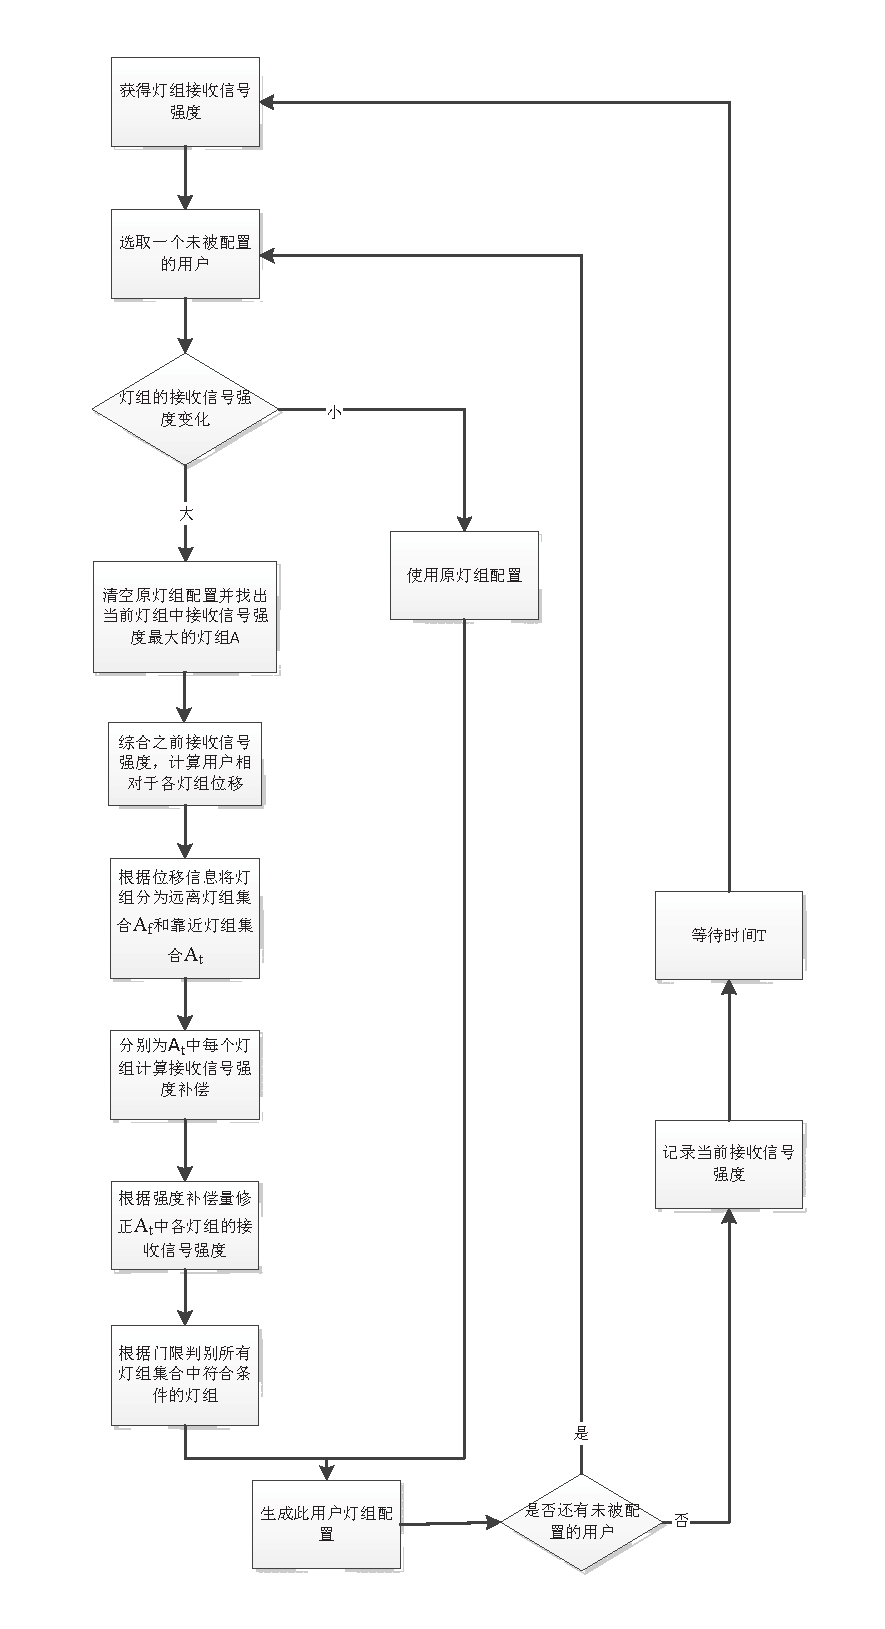
\includegraphics[width=0.8\textwidth]{figures/chapter-4/DistributionSchemeFlow.eps}
	\caption{基于用户运动方向的灯组协同调度算法流程图}
	\label{fig:distribution-scheme-flow}
\end{figure}

如上图所示,算法中的主要过程可以描述如下:

第一步,调度器获得各灯组的反向信道接收信号强度信息;
第二步,选取一个未进行灯组配置的用户,如果每个灯组的接收信号强度变化都在门限值$\Delta P$之内,则直接使用原灯组配置,并进入第八步,如果存在一个灯组的接收信号强度变化超过门限值$\Delta P$则清空原灯组配置信息;
第三步,调度器根据当前的接收信号强度测量结果和前一次灯组配置时的接收信号强度测量结果,通过式()计算出用户在这段判决周期中相对于灯组$A_{i}$移动的位移$\Delta x_{i}$:
第四步,在所有灯组中,将位移$\Delta x_{i}$为正的灯组归为靠近灯组集合$A_{t}$,将位移$\Delta x_{i}$为负的灯组归为远离灯组集合$A_{f}$;
第五步,对于靠近灯组集合$A_{t}$集合中的灯组,利用方向信息$\Delta x_{i}$按如下公式计算出强度修正值 ;
第六步,对靠近灯组集合$A_{t}$中第$i$个灯组的接收信号强度$P_{i}$按照下式进行修正,得到修正后的接收信号强度值$\overline{P_{i}}$;
第七步,判断靠近灯组集合$A_{t}$集合中修正后的接收信号强度值$\overline{P_{i}}$是否满足\eqref{equ:user-enter-hy},若满足则将对应灯组i记入灯组配置结果集合中;同时,判断远离灯组集合 中没有经过修正的灯组接收信号强度是否满足\eqref{equ:user-enter-hy},将满足条件的灯组记入灯组配置结果集合中;
第八步,生成此用户的灯组配置集合,判断当前是否还有未配置的用户,若有未配置的用户,返回第二步,否则,当前获得的修正前的灯组接收信号强度数据放入数据库中;
第九步,调度器等待一个调度时间周期$T$,返回第一步进入下一次灯组调度流程。

\section{仿真实验及结果分析}
为了验证本文所提出的基于用户运动方向的灯组协同调度算法的有效性,本文在NS2平台上搭建了室内可见光通信的平台,并通过修改了NS2底层的源代码进行算法的性能仿真。
为了与本文提出的方法进行对照,在实际的仿真中,也使用了另外两种调度算法进行对照实验。一种调度算法为非协作的最优灯组选择算法,即在灯组的选择过程中,总
是选取接收强度最大的那个灯组,也就意味着是距离用户最近的那个灯组。另外一种调度算法为可用灯组协作的灯组选择算法,即依据当前获得的灯组接收功率,选择那些可以为用户提供服务的灯组组成灯组集为用户提供服务。

仿真中的场景设置为在一个房间内安装有四个灯组,由于系统对单个用户和对多个用户的调度过程是相同的,因此,可以假设一个用户在场景中进行按照如下轨迹进行运动。

\begin{figure}[htbp]
    \centering
	\includegraphics[width=0.8\textwidth]{figures/chapter-4/DistributionUserMove.eps}
	\caption{仿真中的用户运动轨迹图}
	\label{fig:distribution-user-move}
\end{figure}

在本文仿真中,假设用户沿着上述的位置进行移动,已验证算法对用户移动性的支持。灯组的调度算法主要目的就是使用最为合适的灯组为用户服务,从而避免使用全部的灯组进行数据传输,造成资源的消耗。
而当用户处于某灯组的正下方附近时,其光接收功率是比较强的,传输性能也较好,所以灯组的调度其实质就是解决用户处于灯组的边缘区时,多个灯组协同工作进行数据传输这个问题。
所以,为了验证调度性能的好坏,本文仿真中使用灯组的数据重传次数来定量地衡量系统的性能。灯组发生数据的重传就意味着当前的灯组和用户的数据通信存在问题,大量的数据重传发生则意味着用户的当前的通信质量较差。

\subsection{最大修正门限值对算法的影响}
由于算法中使用了接收信号强度补偿,其每个灯组的强度补偿量与最大强度补偿量有关,为了研究最大强度补偿量对算法性能的影响,本文在调度时间为0.6s,
用户的速度为1m/s的情况下,进行了仿真,其中最大修正门限值分别取迟滞门限的0-5倍。得到的结果如下:

\begin{figure}[htbp]
    \centering
	\includegraphics[width=0.8\textwidth]{figures/chapter-4/DistributionBiggestModify.eps}
	\caption{最大修正门限值对系统性能的影响}
	\label{fig:distribution-biggest-modify}
\end{figure}

从上图中可以发现,随着最大修正门限值的增大,数据重传次数先开始下降,在1.5倍之后开始趋于一个稳定值。
这是因为随着最大修正门限值的增大,用户前进方向的灯组的强度修正也就相应增大,这样可以使得在用户未到达某些灯组前,就将该灯组的数据传输通道打开,
当灯组一进入该灯组范围就可以接收服务,但是随着修正门限值的不断增大,虽然灯组的打开时间不断被提前,使得用户在距离该灯组的很远的位置灯组就被打开,
但是灯组在之后的时间内并不能服务到该用户,而需等到用户进入后才能进行系统传输,所以灯组的过早的协作并不能减少数据重传。在下文的仿真中,最大修正门限值取2倍于迟滞门限值。

\subsection{不同的灯组半功率角系数下各算法性能的比较}
在进行LED灯组组网中,灯组的种类选择对最终组网的质量有着重要的影响,而灯组的种类选择主要体现在灯组的半功率角系数这个参数上。灯组的半功率角系数是由灯组的半功率角定义的

\begin{equation}
    m =  - \frac{{\ln 2}}{{\ln (cos{\Phi _{1/2}})}}
\end{equation}

其中,$\Phi _{1/2}$就是灯组的半功率角,代表灯组在包含主瓣最大辐射法相的某一个平面内,相对最大辐射方向功率通量密度下降到一半处的方向和最大辐射方向的夹角。该值可以表征灯组的聚光程度,不同种类的LED灯其半功率角不同。

在本文的仿真中,在不同的半功率角系数下仿真了三种算法在数据重传次数方面的表现,其仿真结果如下所示

\begin{figure}[htbp]
    \centering
	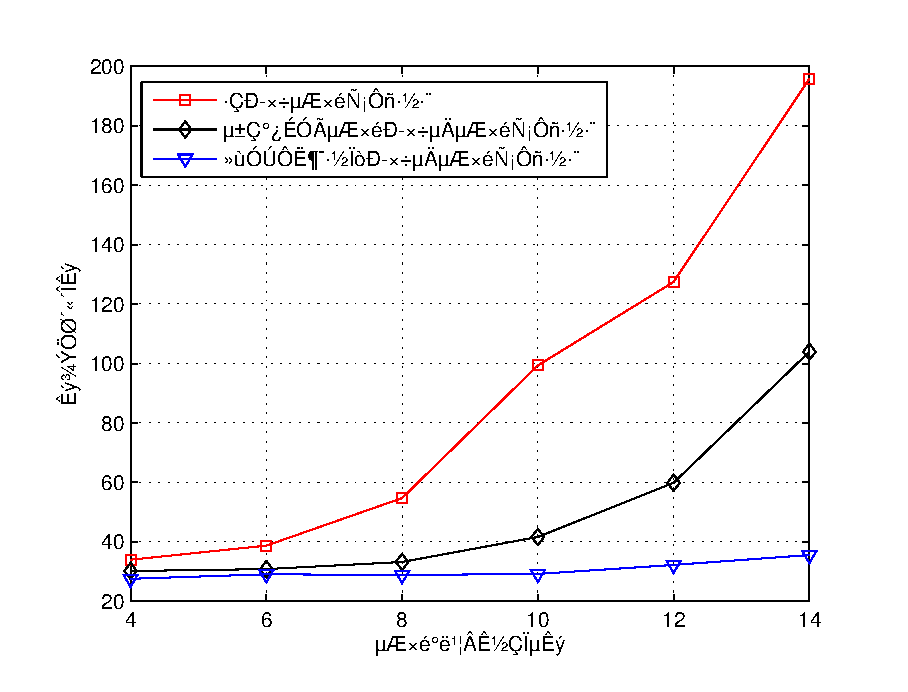
\includegraphics[width=0.8\textwidth]{figures/chapter-4/DistributionLedParam.eps}
	\caption{灯组半功率角系数对系统性能的影响}
	\label{fig:distribution-led-param}
\end{figure}

当m值较小时,也就意味着灯组的半功率角较大,此时灯组的功率辐射较为分散,在灯组的边缘区也有很好的接收功率强度,可以从图上看到,
此时的三种算法得到的数据重传次数都较少,也就意味着系统的性能都较好,因为在这种情况下,三种不同的算法不管有没有进行灯组协作,
都可以在重叠覆盖的边缘区获得较好的通信质量,而采用灯组协作的后两种算法性能会略优越于非协作的算法。随着m值的增加,灯组的半功率角逐渐减小,
也就意味着灯组的功率辐射变得更加集中,因此,此时在灯组的边缘区用户的光接收功率将大大降低。所以从上图中可以看到,这种情况下,若使用非协作算法,
用户在灯组边缘区的通信质量将会非常差,在使用可用灯组进行协作之后,数据重传量将会大幅降低,但是由于其调度的局限性,其协作性能仍然较差。
而在使用本文基于方向的灯组协同调度算法后,显著提高了灯组的协同调度效果,使得系统的通信质量得到进一步的提升。

\subsection{不同的接收视场角下各算法性能的比较}
同样对系统的仿真系统存在影响的还有用户的接收视场角视角(field of view, FOV),用户的接收视场角将会影响灯组的覆盖范围,从而改变用户移动时对灯组的调度。本文在调度时间为0.6s,用户的速度为1m/s的情况下,分别对FOV从30度到60度进行了仿真,以研究其对于算法性能的影响。

\begin{figure}[htbp]
    \centering
	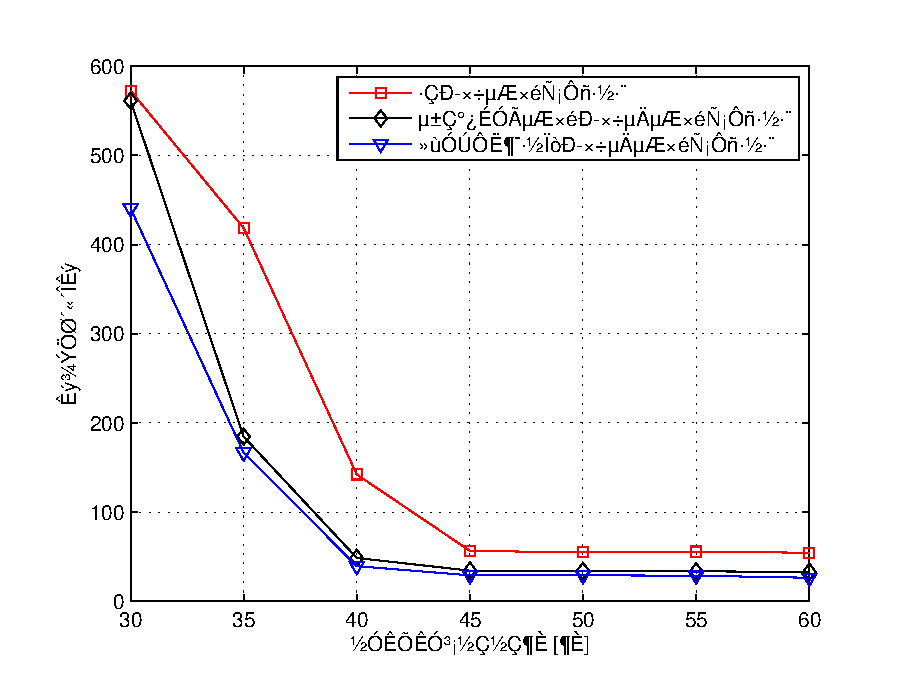
\includegraphics[width=0.8\textwidth]{figures/chapter-4/DistributionUserFov.eps}
	\caption{接收视场角对系统性能的影响}
	\label{fig:distribution-user-fov}
\end{figure}

上图展示了三种不同的灯组调度算法在不同的FOV的情况下的性能变化。可以看到,随着FOV的增大,三种算法的数据重传都出现大幅地减少,这是由于当灯组的FOV较小时,灯组的重叠区覆盖就很小,
用户在灯组的边缘不太容易获得灯组的协作,就算在用户在边缘区得到灯组的协作,其协作效果也并不理想。但是当FOV增加后,本文的灯组协同调度算法将可以充分利用灯组的共同覆盖,
进行灯组间的协同进行数据传输。但如果FOV持续的增大,系统的性能指标却趋于稳定了。这是因为随着FOV的不断增大,虽然灯组的重叠区变大了,但是由于用户在灯组的正下方附近的灯组核心区本身传输质量就很好,
并不需要其他灯组的协作就能保证很好的数据传输,所以较大的FOV也并不能继续提高系统的性能,另一方面,在室内可见光通信中,广角的LED灯组的研究本身就受到器件水平等方面的限制,不太容易被实现,
所以使用合适的FOV角度对室内光通信的灯组调度具有重要的意义。而对于非协作算法而言,当FOV较小时,运动中的用户易于移动到某个灯组的边缘区,甚至是移动出某一灯组的覆盖区域,
因此,这将导致非协作调度方式在FOV较小的情况的数据重传量将非常大。但FOV逐渐增大之后,用户在边缘区运动时才能在信号质量不佳时,接收到其相邻的信号质量较好的灯组的信号,保证通信质量。
对于当前可用灯组协作的灯组选择算法而言,FOV的增大则可以增加用户在边缘区可以使用的协作灯组数,因此,当FOV增加后其数据重传会大幅下降,但是同样由于其调度的瞬时性,因此其性能没有本文提出的算法优越。

\subsection{不同的系统调度时间下各算法性能的比较}
另外,为了验证本文提出的算法性能,我们在不同的系统调度间隔下比较了本文提出的算法和上述提到的两种算法之间的性能。其结果如下所示

\begin{figure}[htbp]
    \centering
	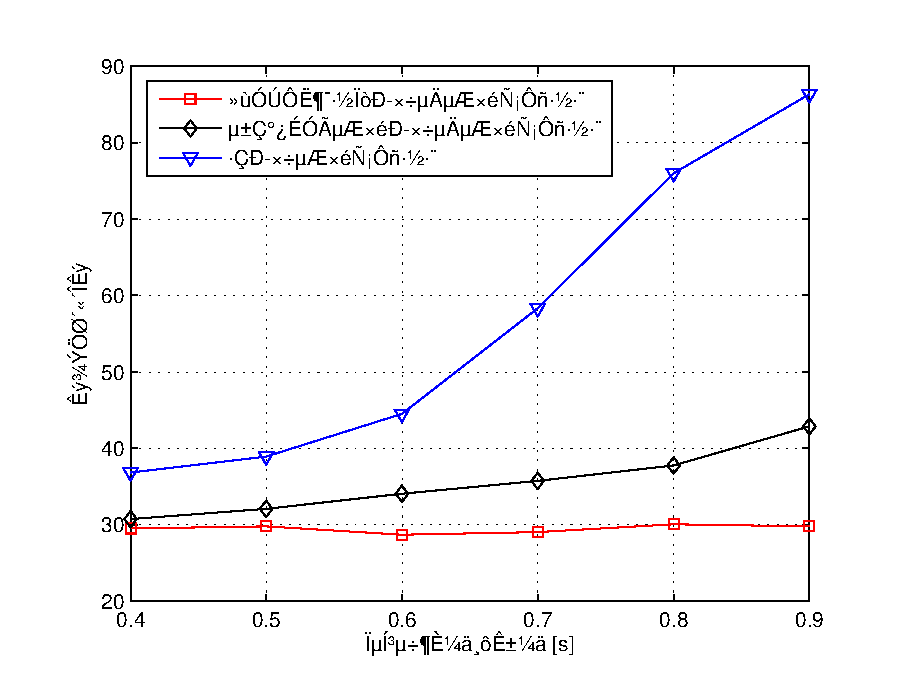
\includegraphics[width=0.8\textwidth]{figures/chapter-4/DistributionSchTime.eps}
	\caption{系统调度时间对系统性能的影响}
	\label{fig:distribution-sch-time}
\end{figure}

从上图中,可以看到,随着系统调度间隔时间的增大,非协作的灯组选择方法的性能将会越来越差,而当前灯组协作的灯组选择方法虽然随着间隔时间增加性能也越来越差,但是其性能优于非协作灯组选择算法。
而本文提出的基于运动方向协作的灯组选择方法随着调度时间的变化波动较小,且性能优于上述两种方法。这是因为系统调度间隔的增大,将会使得调度的周期增加,如果使用非协作灯组选择方法,
用户在边缘区的接收信号质量将会很差,导致大量的重传发生。在使用当前灯组协作的灯组选择方法后,当用户处于边缘区时,若调度及时,多个灯组会协同工作进行下行数据传输,但是如果调度时间过长,
也有可能导致用户不能及时地获得多灯组的协作。而本文提出的基于用户运动方向协作的灯组选择方法,则可以克服上述的弊端,当调度周期很长时,利用对用户的运动方向预测,提前进行灯组的协作,从而提高系统的协作性能。

\subsection{不同的用户移动速度下各算法性能的比较}
在将系统的调度周期设定为0.6s之后,本文又对不同用户运动速度下,系统采用不同的调度方法的情况进行了仿真研究,其结果如下图所示

\begin{figure}[htbp]
    \centering
	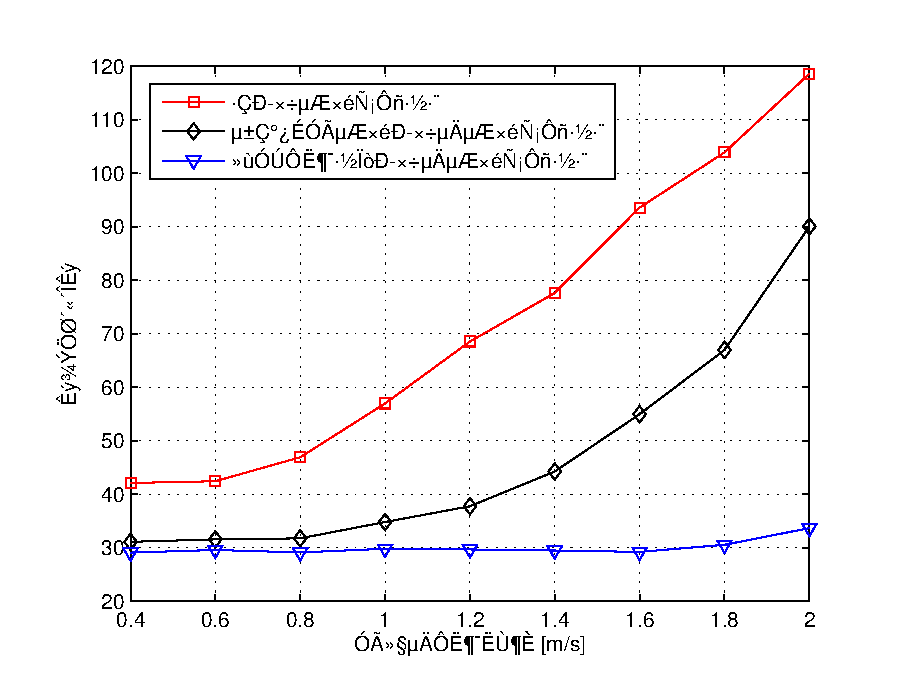
\includegraphics[width=0.8\textwidth]{figures/chapter-4/DistributionUserSpeed.eps}
	\caption{用户移动速度对系统性能的影响}
	\label{fig:distribution-user-speed}
\end{figure}

对于上图,从横向看,可以发现随着用户的移动速度的不断增加,使用三种灯组选择方法的性能都会出现一定程度的恶化。但是非协作灯组选择和当前可用灯组协作这两种方法的系统性能下降较为严重,而对本文提出的基于运动方向协作的方法的性能影响较小。
从纵向对比,可以看到,本文提出的方法的性能要优于另外两种灯组选择方法。在用户的速度达到2m/s时,数据重传次数只有非协作灯组选择方法的约25\%,是当前可用灯组选择方法的30\%。
这是因为随着用户速度的增加,若采用非协作灯组选择方法,用户在调度周期中将会更有可能移动出原先调度灯组的覆盖范围,且由于非协作灯组选择只使用一个灯组服务用户,边缘区的信号质量会很差,所以非协作灯组选择方法的系统性能是最差的。
而当我们采用了当前可用灯组协作的灯组选择方法后,虽然用户在边缘区会受到多个灯组的协同工作进行数据传输,但是较快的用户移动仍然可能会引起用户移动出原先调度的灯组集,使得系统系能指标得不到保障。
但在使用了本文提出的灯组选择方法后,由于在灯组的调度时,由于增加了用户的位置信息,可以在灯组的调度中包含了将来可以使用中的灯组,从而避免由于用户的移动造成的用户在调度周期内在边缘区重传次数过高的问题。

\section{本章小结}	
本章主要研究了在分布式灯组布局下的灯组协同调度问题。这里的分布式灯组布局是指,所有的灯组只负责物理层的数据传输工作,而不涉及具体的用户控制等功能,而数据的传输控制由连接各灯组的调度器负责。
本章首先介绍了分布式灯组布局的概念,并介绍了本章所提及系统的上下行信道,多用户通信方式等内容,在此基础上,本章利用用户进行数据传输时的功率测量,提出了一种基于用户方向的灯组协同调度算法,在进行灯组的调度时,
不仅考虑测量到的用户的上行功率,并考虑到用户的移动方向,从而获得更加准确的调度灯组,当用户移动到灯组的边缘区时通过调度好的灯组协同进行下行数据传输。最后,本章在NS2平台上进行了算法的仿真,并和另外两种灯组调度算法进行了对比,
仿真结果表明,本文提出的算法在灯组边缘区可以获得更好的灯组协作效果,对比其他两种调度算法有着较大的优势。
